%%%%%%%%%%%%%%%%%%%%%%%%%%%%%%%%%%%%%%%%%%%%%%%%%%%%%%%%%%%%%%%%%%%%
%% I, the copyright holder of this work, release this work into the
%% public domain. This applies worldwide. In some countries this may
%% not be legally possible; if so: I grant anyone the right to use
%% this work for any purpose, without any conditions, unless such
%% conditions are required by law.
%%%%%%%%%%%%%%%%%%%%%%%%%%%%%%%%%%%%%%%%%%%%%%%%%%%%%%%%%%%%%%%%%%%%



\documentclass{beamer}
\usetheme[faculty=fi]{fibeamer}
\usepackage[utf8]{inputenc}
\usepackage[
   main=english, %% By using `czech` or `slovak` as the main locale
                        %% instead of `english`, you can typeset the
                        %% presentation in either Czech or Slovak,
                        %% respectively.
   czech, slovak, greek %% The additional keys allow foreign texts to be
]{babel}            %% typeset as follows:

%%
%%    \begin{otherlanguage}{czech}    ... \end{otherlanguage}
%%    \begin{otherlanguage}{slovak}   ... \end{otherlanguage}
%%


%% These macros specify information about the presentation
\title{Sampling the flux space of microbial metabolic networks
% for (un)biased assessment of the possible functional states
} %% that will be typeset on the
\subtitle{the example of SARS-CoV-2 on the human alveolar macrophage metabolic network} %% title page.
\author{Haris Zafeiropoulos} 

%% These additional packages are used within the document:
\usepackage{ragged2e}   % `\justifying` text
\usepackage{booktabs}   % Tables
\usepackage{tabularx}
\usepackage{tikz}         % Diagrams
\usetikzlibrary{calc, shapes, backgrounds}
\usepackage{amsmath, amssymb}
\usepackage{url}          % `\url`s
\usepackage{listings}   % Code listings
\usepackage{setspace}

\frenchspacing

\begin{document}

   \shorthandoff{-}
   \frame[c]{\maketitle}


   % Print an outline at the beginning of sections

   % 1st section using dark frames
   % \begin{darkframes}

   % \begin{darkframes}
   % SLIDE 2
   \begin{frame}{Genome-scale metabolic reconstruction}
      
      \begin{singlespace}
         \begin{tikzpicture}[overlay,remember picture]
            \node[anchor=north west, xshift=30pt,yshift=-50pt]
               at (current page.north west) {
                  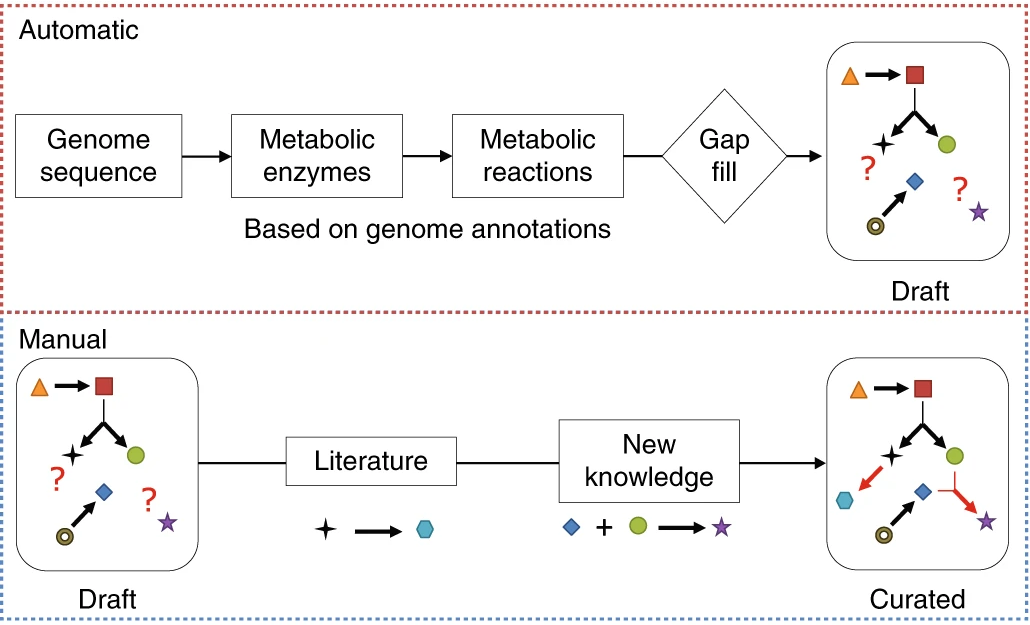
\includegraphics[width=110mm]{resources/building_gmd.png}
               };
            \node[align = left, above] at (current page.south) {
               \scriptsize 
               Figure from: Heirendt, Laurent, et al. "Creation and analysis of biochemical  \\ 
               \scriptsize
               constraint-based models using the COBRA Toolbox v. 3.0. Nature protocols 14.3 (2019): 639-702."
            };
         \end{tikzpicture}
      \end{singlespace}
      % \captionof{figure}{\textbf{Confusion Matrix}}

   \end{frame}

   
   % SLIDE 3
      % \bigskip ; \justifying ; \bigskip

      \begin{frame}{From a stoichiometric matrix}
         \framesubtitle{to a constraint-based model}
         
         \begin{singlespace}
            \begin{tikzpicture}[overlay,remember picture]

               \node[anchor=north west, xshift=20pt,yshift=-65pt]
                  at (current page.north west) {
                     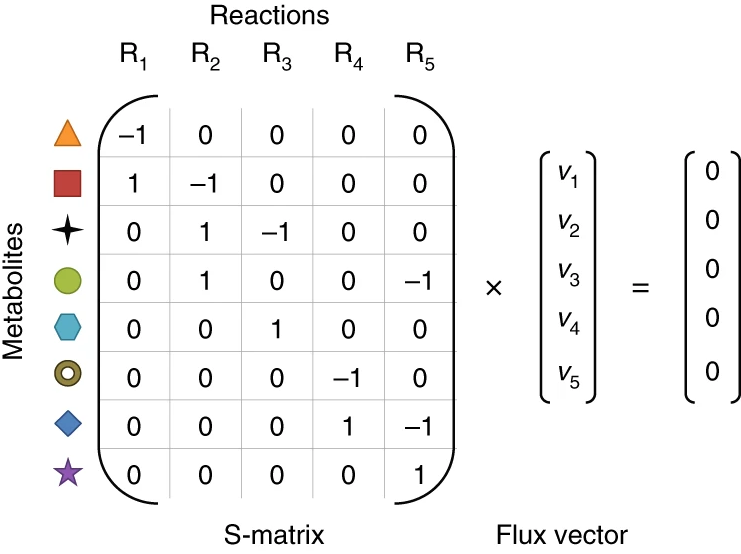
\includegraphics[width=70mm]{resources/stoichiometric_matrix.png}
                  };

               \node[align = left, above] at (current page.south) {
                     \scriptsize \
                     Figure from: Heirendt, Laurent, et al. "Creation and analysis of biochemical  \\ 
                     \scriptsize
                     constraint-based models using the COBRA Toolbox v. 3.0. Nature protocols 14.3 (2019): 639-702."
               };

               \node[align = center, left, xshift=-10pt] at (current page.east) {
                  \small
                  \textbf{Flux Balance Analysis}
                  \\ 
                  \small
                  Maximize \/ minimize an \\
                  \small
                  objective function:  \\
                  \small
                  $\psi = c_1 v_1 + c_2 v_2 + .. + c_5 v_5$ \\
                  \small
                  such that: \\
                  \small
                  $S * v = O$ \\ 
                  \small
                  and for each reaction $i$: \\
                  \small
                  $lb_i <= v_i <= ub_i$ \\ 
                  
                  \\

                  \small
                  where $lb$: lower bound, \\
                  \small
                  $ub$: upper bound and \\
                  \small
                  $S$: the stoichiometric matrix
               };

            \end{tikzpicture}
         \end{singlespace}

    
       
      \end{frame}
         


   % SLIDE 4
   \begin{frame}[label=simmonshall]{Flux sampling} 

      \framesubtitle{an alternative approach}
      \begin{singlespace}
         \begin{tikzpicture}[overlay,remember picture]

            \node[anchor=north west, xshift=20pt,yshift=-60pt]
               at (current page.north west) {
                  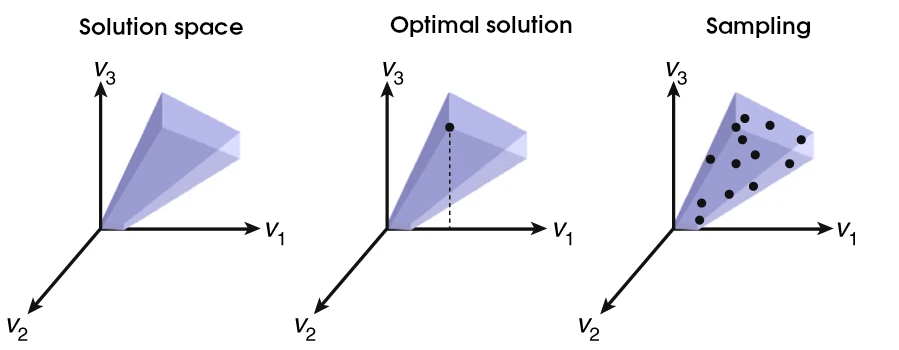
\includegraphics[width=100mm]{resources/solution_spaces.png}
               };

            \node[align = left, above] at (current page.south) {
               \scriptsize \
               Figure from: Heirendt, Laurent, et al. "Creation and analysis of biochemical  \\ 
               \scriptsize
               constraint-based models using the COBRA Toolbox v. 3.0. Nature protocols 14.3 (2019): 639-702."
               };
         \end{tikzpicture}

         % \bigskip ; \justifying ; \bigskip
         \bigskip ; \justifying ; \bigskip
         \bigskip ; \justifying ; \bigskip

         Allows for:
         \begin{itemize}
            \item  analysis of GSMMs without the need of an objective function
            % If we sample a sufficiently large number of points, uniformly distributed, in the polytope,
            % then these correspond to uniformly at random sample of steady states of the metabolic network.
            % In this way we can obtain an overview of all the possible flux values and  generate the probability distribution for each flux.
            % Hence, we obtain a thorough representation of the steady states of the metabolic network and we can
            % study the properties of certain components of the whole network to deduce significant biological insights.
            
         \end{itemize}

      \end{singlespace}


   \end{frame}




   % \begin{frame}[plain,c]
   %    \begin{center}
   %    \Large \textbf{The region of steady states}
   %    \end{center}
   %    %\centerline{The region of steady states}
   %    \begin{columns}
   %    \begin{column}{0.5\textwidth}
   %    \vspace*{0.2cm}
   %    \begin{center}
   %       As a {\color{blue} low dimensional} polytope.\\% in $\mathbb{R}^n$.\\
   %       %\vspace*{0.2cm}
   %       %\includegraphics[scale=0.2]{./figures/low_dim_poly}
   %        \end{center}    
   %        \vspace*{0.2cm}
   %       \begin{equation*}
   %        \begin{split}
   %           &\quad\quad\quad\quad\quad Sv = 0,\\ & \quad\quad\quad\quad v_{lb}\leq v \leq v_{ub} \hspace*{1.6cm} {\color{orange}\stackleftrightarrow{v = Nx}} \\
   %           & \quad\quad\quad S\in\mathbb{R}^{m\times n},\ \mathbf{v}\in\mathbb{R}^n 
   %        \end{split}
   %        \end{equation*}
   %    \end{column}
   %    \begin{column}{0.5\textwidth}  %%<--- here
   %    \vspace*{0.1cm}
   %    \begin{center}
   %    As a {\color{red} full dimensional} polytope\\
   %         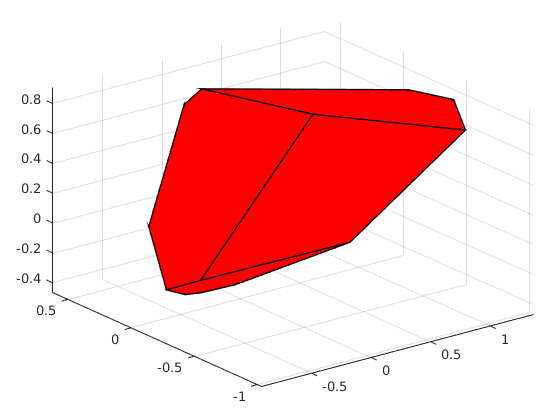
\includegraphics[scale=0.2]{./figures/polytope}\\
   %         $P:=\{ x\in\mathbb{R}^d\ |\ Ax\leq b \}$
   %         \end{center}
   %    \end{column}
   %    \end{columns}
   %    \vspace*{0.3cm}
   %    \begin{align*}
   %    A = \begin{pmatrix} I_n N \\ -I_n N\end{pmatrix}\ \text{and }b = \begin{pmatrix} v_{ub} \\ v_{lb} \end{pmatrix}  N
   %    \end{align*}
   %    %$A = \begin{pmatrix} I_n N \\ -I_n N\end{pmatrix}$
   %    %and $b = \begin{pmatrix} x_{ub} \\ x_{lb} \end{pmatrix}  N$
   %    %\begin{itemize}
   %       \centering $N\in\mathbb{R}^{n\times d}$ the matrix of the right nullspace of $S$.
   %    %\end{itemize}
   %    \end{frame}
      
      
      % %9th slide
      % \begin{frame}[plain,c]
      % \begin{center}
      % \Large \textbf{Sampling steady states}
      % \end{center}
      
      % \begin{columns}
      % \begin{column}{0.5\textwidth}
      % \begin{center}
      %    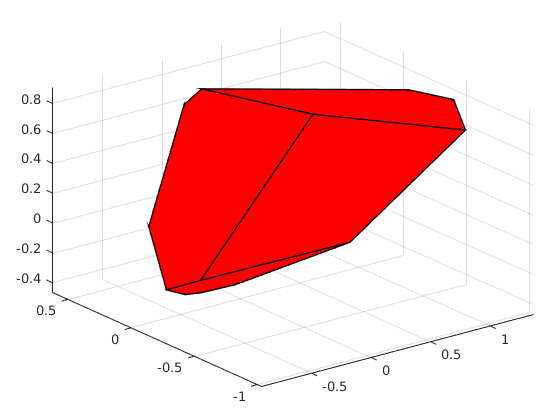
\includegraphics[scale=0.35]{./figures/polytope}
      % \end{center}
      % \end{column}
      % \begin{column}{0.5\textwidth}  %%<--- here
      
      % \begin{center}
      %    \includegraphics[scale=0.35]{./figures/sampling}
      % \end{center}
      % \end{column}
      % \end{columns}
      
      % \begin{itemize}
      %    \item \footnotesize Sampling could lead to important biological insights! {\footnotesize\color{ao} [Palsson'15]}
      %    \item Explore the flux space {\footnotesize\color{ao} [Schellenberger,Palsson'09]}.
      % \end{itemize}
         
      % \begin{mdframed}
      % \begin{center}\
      % \textit{We introduce a\\}
      % \textbf{M}ultiphase \textbf{M}onte \textbf{C}arlo \textbf{S}ampling algorithm\\ based on \textbf{Billiard Walk}
      % \end{center}
      % \end{mdframed}
      % \end{frame}
      

   % Thank you SLIDE
   \begin{darkframes}
   \begin{frame}{Thank you for your attention}
         
      % URLs
      GitHub repository  : \href{https://github.com/GeomScale/dingo/}{https://github.com/GeomScale/dingo/} \\ 
      \bigskip
      email    : \href{haris-zaf@hcmr.gr}{haris-zaf@hcmr.gr} \\
      Twitter  : \href{https://twitter.com/haris_zaf}{haris\_zaf} \\
      web-site : \url{https://hariszaf.github.io/} \\

      % Logos   
      % -------------- 

      % UoC
      \begin{tikzpicture}[overlay,remember picture]
         \node[anchor=south west,
               xshift=-350pt,
               yshift=10pt]
               at (current page.south east) {
                  
\includegraphics[height=17mm]{
                     resources/UoC_logo_white.png
                  }
               };
      \end{tikzpicture}

      % IMBBC
      \begin{tikzpicture}[overlay,remember picture]
         \node[anchor=south east,
            xshift=-185pt,
            yshift=25pt]
            at (current page.south east) {
               
\includegraphics[width=35mm]{resources/logo-imbbc.png}
            };
      \end{tikzpicture}%

      % HCMR
      \begin{tikzpicture}[overlay,remember picture]
         \node[anchor=south east,
               xshift=-125pt,
               yshift=10pt]
               at (current page.south east) {
                  
\includegraphics[height=20mm]{
                     resources/hcmr-logo.png
                  }
               };
      \end{tikzpicture}%

      % GeomScale
      \begin{tikzpicture}[overlay,remember picture]
         \node[anchor=south east,
               xshift=-5pt,
               yshift=22pt]
               at (current page.south east) {
                  
\includegraphics[width=40mm]{
                     resources/geomscale-logo.png
                  }
               };
      \end{tikzpicture}

   \end{frame}
   \end{darkframes}

\end{document}
